\documentclass[graphics]{beamer}

\usepackage{graphicx}
\usepackage{verbatim}
\usepackage{wrapfig}
\useoutertheme{shadow}
%\usecolortheme{orchid}
\usecolortheme{seahorse}


% math commands
\newcommand{\be}{\begin{eqnarray}}
\newcommand{\ee}{\end{eqnarray}}
\newcommand{\beq}{\begin{equation}}
\newcommand{\eeq}{\end{equation}}
\def\simless{\mathbin{\lower 3pt\hbox
      {$\rlap{\raise 5pt\hbox{$\char'074$}}\mathchar"7218$}}}
\def\simgreat{\mathbin{\lower 3pt\hbox
      {$\rlap{\raise 5pt\hbox{$\char'076$}}\mathchar"7218$}}} %> or of order

% variables

\def\toonscale{0.45}
\def\mboxy#1{\mbox{\small #1}}


\begin{comment}
\AtBeginSection[]{
  \frame{
    \frametitle{Outline}
    \tableofcontents[currentsection]
  }
}
\end{comment}

\title{Tale of two Tensors
}
\subtitle{}
\author[U. Pen]{\textcolor{green}{Ue-Li Pen, Haoran Yu, Pavel Motloch}
\\[8mm] 
}
\date{January 28, 2020}


\begin{document}

\frame{
\begin{picture}(320,250)
\put(-50,-130){
\includegraphics[width=5.5in]{Figures/delta_nu_sim.pdf}}
\end{picture}
\vspace{-3in}
\titlepage
}

%\section*{Introduction}
\section{Tale of two Tensors}

\begin{comment}
  \subsection{Outline}

  \frame{
    \frametitle{Outline}
    \tableofcontents
  }
\end{comment}


  \frame{
    \frametitle{Introduction}
    \begin{itemize}
        \item Towards the beginning: initial tidal shear
        \item Galaxy spins are fossils of IC
        \item Simulations: angular momentum directions of TTT, DM,
          Baryons very well aligned.  Magnitudes poorly predicted, and
          not observable
        \item New: measuring and predicting oriented spin
     \end{itemize}
}


\frame{
    \frametitle{Prograde Winding}
\includegraphics[width=4.1in]{Figures/M51s.jpg}  

(M51, from Wikipedia)
  }
\frame{
    \frametitle{Tilt}
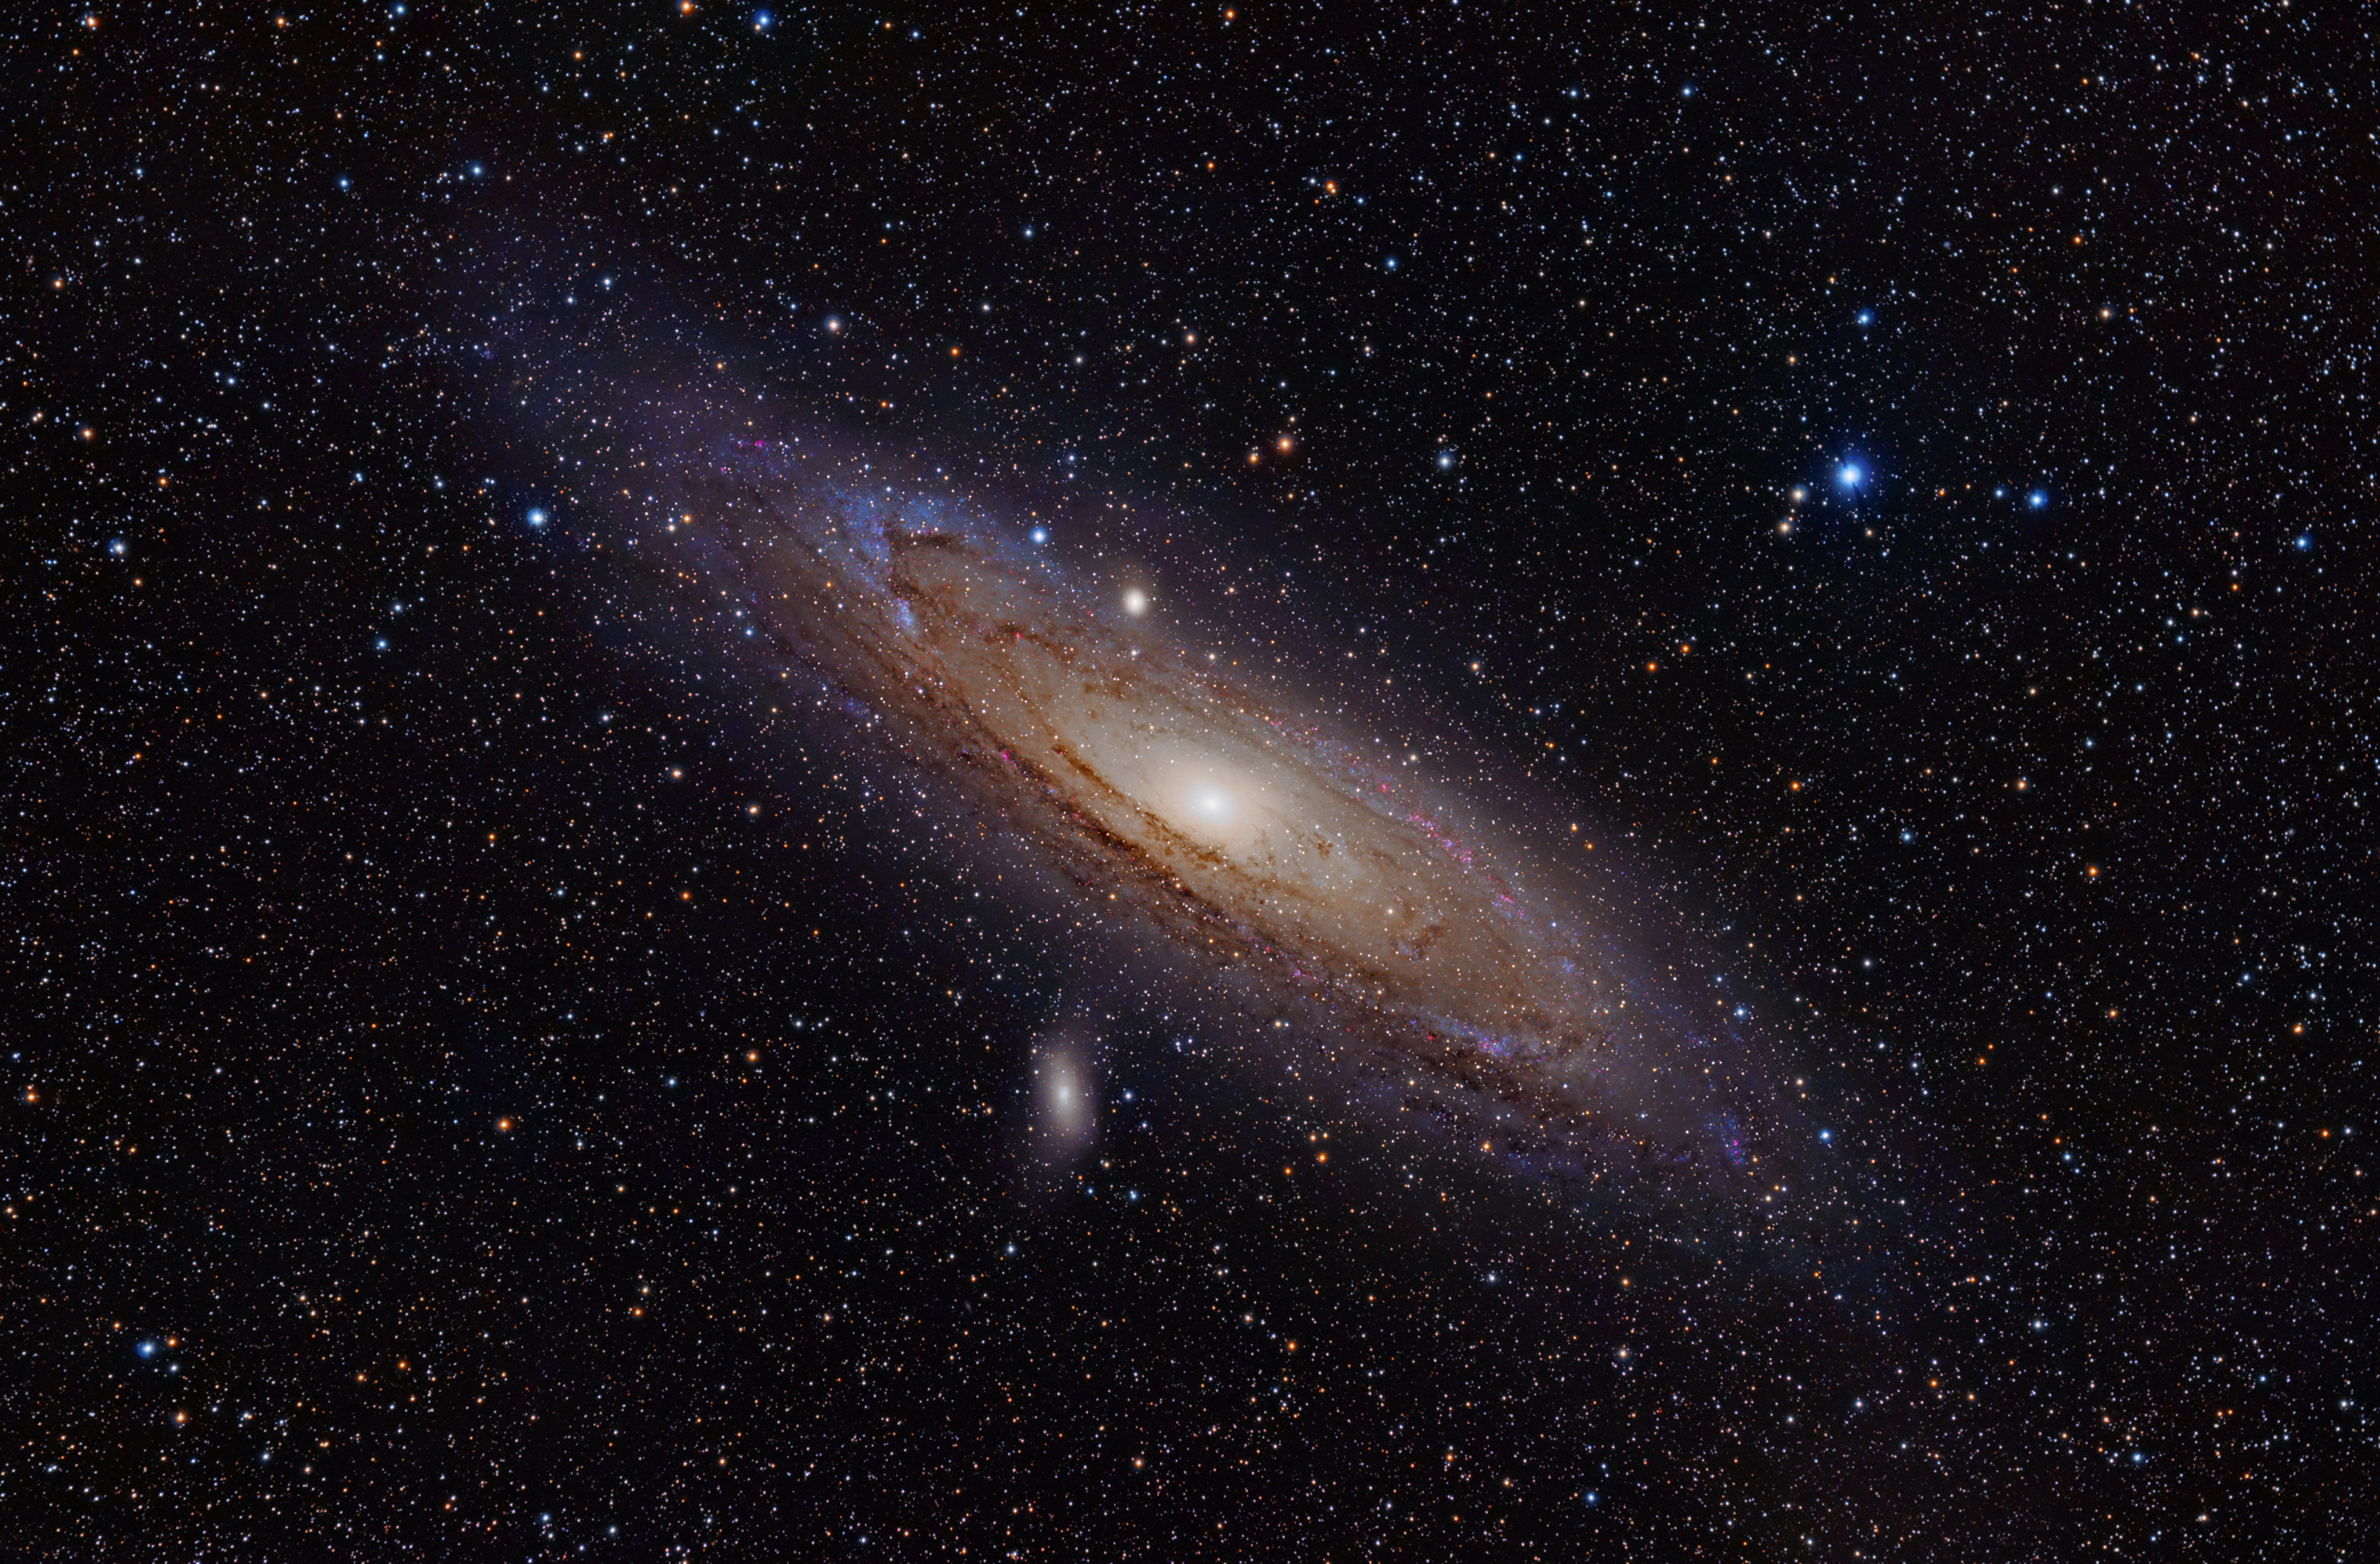
\includegraphics[width=4.1in]{Figures/AndromedaGalaxy.jpg}  

(M31, from Wikipedia)
  }

  \frame{
    \frametitle{Galaxy Spins}
    \begin{itemize}
        \item most galaxies are rotating disks of stars and gas
        \item readily identifyable spin axis
        \item dust lanes, trailing spiral arms, (HI) velocity (rotation) field
     \end{itemize}
}

  \frame{
    \frametitle{Observables}
    \begin{itemize}
        \item ellipticity
        \item position angle
        \item winding direction (S vs Z)
        \item reddening
        \item human and machine classifications for $10^{4-6}$ objects
          (galaxy zoo, Land+ 2008 )
    \end{itemize}
}


\frame{
    \frametitle{Zoo}
\includegraphics[width=4.1in]{Figures/land2008.png}  
  }

  \frame{
    \frametitle{Context}
    \begin{itemize}
        \item S White 1984: TTT
        \item Genel++: spin magnitude
        \item Lee\&Pen 2000: LSS statistical theory
        \item Yu++ 2018: Lagrangian theory, high fidelity direction
          memory, poor magnitude memory
     \end{itemize}
}


  \frame{
    \frametitle{Angular momentum}
    \begin{itemize}
        \item 1st order effect from misalignment of moment of inertia
          and tidal tensor
        \item torque: $\tau\equiv\int \rho \bf{r} \times \nabla \phi$
        \item Taylor expand: $\tau_i=\epsilon_{ijk} \int \rho x^jx^l \partial_l\partial_k\phi \equiv\epsilon_{ijk} I_{il}T_{lk}$
        \item Tensor form $\tau= * I \cdot T$
        \item first realized by S. White (1984), see also LP00
     \end{itemize}
}

\frame{
    \frametitle{3-D: E-mode}
%\vspace{-0.5in}
\hspace{-0.2in}\includegraphics[width=2.3in]{Figures/nonlinear.png}  
\vspace{0.15in}\includegraphics[width=2.21in]{Figures/reconstructed.png}  

Eulerian (L) vs Lagrangian (R) (from Yu et al 2016, 1610.7112)
  }

  \frame{
    \frametitle{Tensors}
    \begin{itemize}
        \item Tide: ${\bf T}$ reconstructed from density field
        \item Inertia: non-linear reconstruction of ${\bf I}$
        \item strongly correlated
     \end{itemize}
}
\frame{
    \frametitle{Sim}
\includegraphics[width=4.1in]{Figures/I-T.png}  
Yu+2018
  }

\frame{
    \frametitle{Lagrangian coordinates}
\center{\includegraphics[width=4.3in]{Figures/delta_reco_raw.pdf}  }
  }
\frame{
\vspace{-0.5in}
    \frametitle{Reconstruction}
    \begin{itemize}
        \item multiple successful approaches
        \item injective Isobaric (Pen++ 1995, Zhu/Wang/Yu/ 2016-2020 )
        \item ELUCID, Schmidtful17,  Shi18, Hada18, Hikage19, etc
        \item typically achieve 50\% phase fidelity per mode up to
          $k\sim 1h$/Mpc.
     \end{itemize}
  }
\frame{
\vspace{-0.5in}
    \frametitle{What about Inertia Tensor?}
    \begin{itemize}
        \item $I$ readily measured in simulations
        \item highly correlated with tide $T$
        \item depends on small misalignment with {\it external} shear
        \item use small scale tide as proxy for inertia, and larger
          scale for tide
     \end{itemize}
  }


\frame{
\vspace{-0.5in}
    \frametitle{Conclusions}
    \begin{itemize}
      \item Galaxy spin determined by cosmic structure: Tide and Inertia
      \item Partially reconstructable from non-linear cosmic web: two scale tensors
      \item Direction readily observed and well preserved in
        non-linear evolution
      \item Initial detection in ELUCID-zoo comparison
          \item parity odd field, less likely to be contaminated
            (e.g. lensing)
     \end{itemize}
  }


\end{document}
